%~~~~~~~~~~~~~~~~~~~~~~~~~~~~~~~~~~~~~~~~~~~~~~~~~~~~~~~~~~~~~~~~~~~~~~~~~~~~~~~~~
\chapter{EPAS LPV model}
\label{chap_epas_lpv_model} 
% Approx. 5 pages

%~~~~~~~~~~~~~~~~~~~~~~~~~~~~~~~~~~~~~~~~~~~~~~~~~~~~~~~~~~~~~~~~~~~~~~~~~~~~~~~~~
\section{Introduction}

In the previous Chapter \ref{chap_linear_parameter_varying_modeling_and_stability}, we discussed LPV systems. We will continue in this chapter with a brief introduction to EPAS systems and the application of the LPV model to EPAS systems.

EPAS is an electrical power assistance system that can supply power assistance on demand. This system is replacing the hydraulic pistons with electric motors in order to push the steering rack. This method of steering is directly eliminating some outdated problems such as the uneven pressure of the pistons

%TODO you left here continue from here.




There are different types of EPAS systems depending on the market requirements and the application ares. Some of these systems are column drive where the electric motor is positioned vertically to the steering column.

%~~~~~~~~~~~~~~~~~~~~~~~~~~~~~~~~~~~~~~~~~~~~~~~~~~~~~~~~~~~~~~~~~~~~~~~~~~~~~~~~~
\section{System overview}
\label{sec_system_overview}

The parallel-mounted power assist steering (ParPAS) system is an electro-mechanical rack and pinion power assisted steering system for a front-steered passenger car. The electric motor is positioned parallel to the rack and driven by a belt and a recirculating ball screw drive transmission, as shown in Figure~\ref{fig_parpas_model}.

The steering system consists of the following: a steering column, a steering wheel, a torque sensor (TSS) with a controller area network (CAN) interface, a rack and pinion steering gear, a 3-phase permanent magnet synchronous brushless DC electric motor (equipped with an angle sensor), a belt transmission and a recirculating ball screw drive transmission, an electronic control unit (ECU), and two tie rods. The ECU has a vehicle and a private CAN interface~\citep{paholics2006epas}.

%TODO Try gray scale pictures 
\begin{figure}[b]
	\begin{center}
		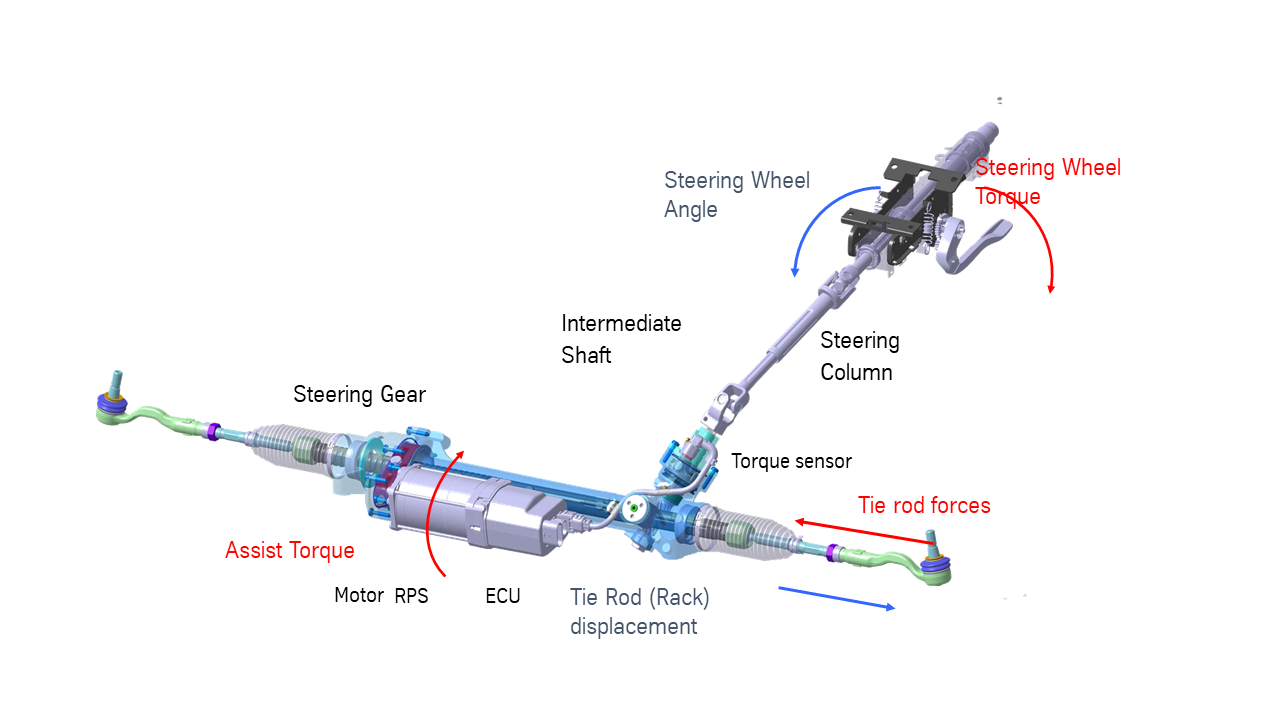
\includegraphics[width=105mm]{figures/parpas_model.png}
		\caption{Model of the parallel-mounted EPAS system~\citep{benyo2013eps}.}
		\label{fig_parpas_model}
	\end{center}
\end{figure}

%~~~~~~~~~~~~~~~~~~~~~~~~~~~~~~~~~~~~~~~~~~~~~~~~~~~~~~~~~~~~~~~~~~~~~~~~~~~~~~~~~
\section{Model reduction}
\label{sec_model_reduction}

In control design, reduced linear models are used to ease the design and simplify complex systems like the steering system of a car.

In order to obtain the simplified linear model with 2 degrees of freedom, the inertia of the wheel, rack, ball screw, tie rods, and motor has to be reduced to the pinion. The related disturbances, frictions, and damping also have to be transferred to the pinion.

The motor inertia is reduced to the pinion as follows:

\begin{align}
	\begin{split}
		J_{red} = J_{motor} 
		\cdot \Bigg( \frac{i_{belt} \cdot i_{screw}}{i_{pinion}} \Bigg)^{2} 
		+ J_{screw} \cdot \Bigg( \frac{i_{screw}}{i_{pinion}} \Bigg)^{2} \\
		+ (m_{rack} + m_{tierods}) \cdot \Bigg( \frac{1}{i_{pinion}} \Bigg)^{2} \\
		+ 2 \cdot J_{wheel} \cdot 
		\Bigg( \frac{1}{i_{frame} \cdot i_{pinion}} \Bigg)^{2}
	\end{split}
\end{align}

The motor damping is reduced to the pinion as follows:

\begin{align}
	b_{red} 
	= b_{motor} \cdot \Bigg(\frac{i_{belt} \cdot i_{screw}}{i_{pinion}}\Bigg)^{2}
	+ b_{screw} \cdot \Bigg(\frac{i_{screw}}{i_{pinion}}\Bigg)^{2} 
	+ b_{rack} \cdot \Bigg(\frac{1}{i_{pinion}}\Bigg)^{2}
\end{align}

The result of this model reduction is the simplified linear model, which is a damped mass-spring system with two degrees of freedom as shown in Figure~\ref{fig_red_lin_model}.

The following symbols are used as notations in the figure: The $J_{up}$ is the reduced inertia of the motor, screw, wheel, rack, and tie rods, and the $J_{red}$ is the inertia of the steering wheel. In between them, there are the steering column inner damping ($b_{sensor}$) and the steering column stiffness ($c_{sensor}$), which primarily consists of the torque sensor (torsion bar) stiffness. The $b_{up}$ viscous coefficient of the steering wheel friction; the $b{red}$ is the reduced damping of the motor, screw, and rack.

The system input is the required motor torque ($T_{motor}$), and the disturbances are the driver torque ($T_{driver}$) and the load ($T_{load}$). The measurements of the system are the outputs. The motor angle speed ($i_{gear} \cdot \omega_{pinion}$), and the steering column torque ($c_{sensor} \cdot \Delta \varphi$).

\begin{figure}[b]
	\begin{center}
		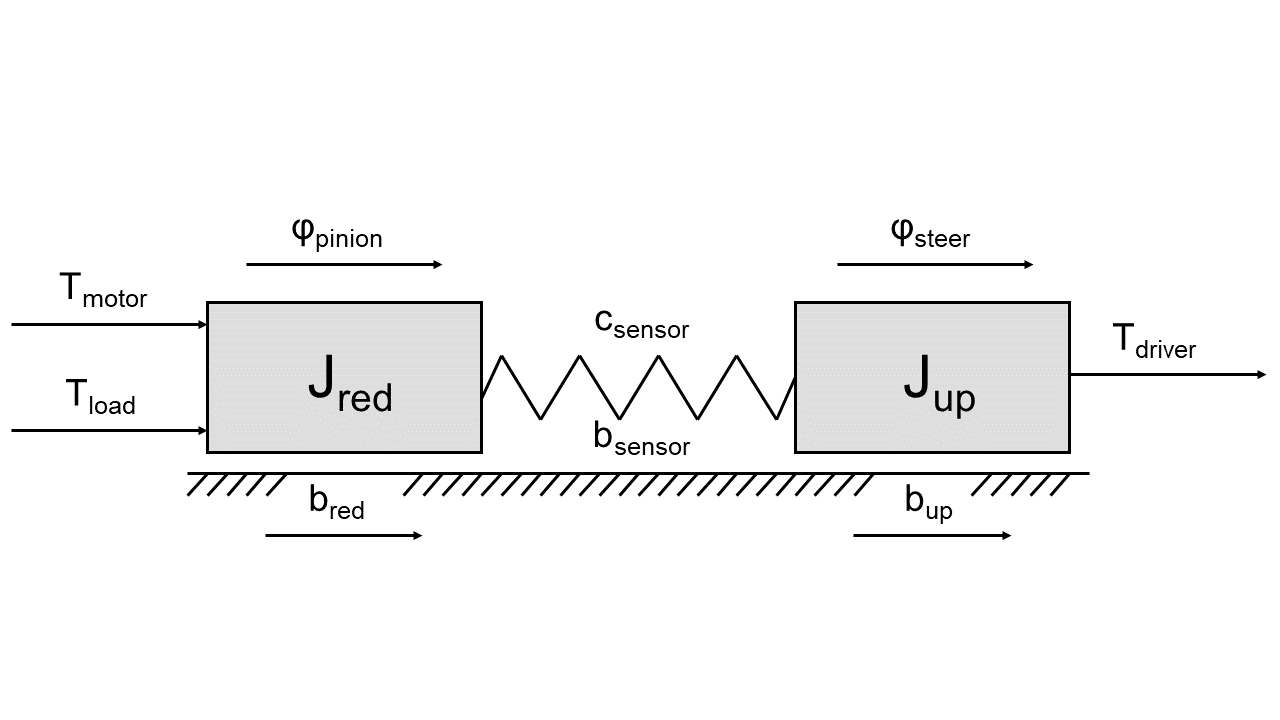
\includegraphics[width=100mm]{figures/red_lin_model.png}
		\caption{Reduced linear model of the EPAS 
		system~\citep{paholics2006epas}.}
		\label{fig_red_lin_model}
	\end{center}
\end{figure}

